\documentclass[]{article}
\usepackage{lmodern}
\usepackage{amssymb,amsmath}
\usepackage{ifxetex,ifluatex}
\usepackage{fixltx2e} % provides \textsubscript
\ifnum 0\ifxetex 1\fi\ifluatex 1\fi=0 % if pdftex
  \usepackage[T1]{fontenc}
  \usepackage[utf8]{inputenc}
\else % if luatex or xelatex
  \ifxetex
    \usepackage{mathspec}
  \else
    \usepackage{fontspec}
  \fi
  \defaultfontfeatures{Ligatures=TeX,Scale=MatchLowercase}
\fi
% use upquote if available, for straight quotes in verbatim environments
\IfFileExists{upquote.sty}{\usepackage{upquote}}{}
% use microtype if available
\IfFileExists{microtype.sty}{%
\usepackage{microtype}
\UseMicrotypeSet[protrusion]{basicmath} % disable protrusion for tt fonts
}{}
\usepackage[margin=1in]{geometry}
\usepackage{hyperref}
\hypersetup{unicode=true,
            pdftitle={CSC8631 : Data Management and Explore Data Analysis------Online Learning},
            pdfauthor={Minye Shao},
            pdfborder={0 0 0},
            breaklinks=true}
\urlstyle{same}  % don't use monospace font for urls
\usepackage{longtable,booktabs}
\usepackage{graphicx}
% grffile has become a legacy package: https://ctan.org/pkg/grffile
\IfFileExists{grffile.sty}{%
\usepackage{grffile}
}{}
\makeatletter
\def\maxwidth{\ifdim\Gin@nat@width>\linewidth\linewidth\else\Gin@nat@width\fi}
\def\maxheight{\ifdim\Gin@nat@height>\textheight\textheight\else\Gin@nat@height\fi}
\makeatother
% Scale images if necessary, so that they will not overflow the page
% margins by default, and it is still possible to overwrite the defaults
% using explicit options in \includegraphics[width, height, ...]{}
\setkeys{Gin}{width=\maxwidth,height=\maxheight,keepaspectratio}
\IfFileExists{parskip.sty}{%
\usepackage{parskip}
}{% else
\setlength{\parindent}{0pt}
\setlength{\parskip}{6pt plus 2pt minus 1pt}
}
\setlength{\emergencystretch}{3em}  % prevent overfull lines
\providecommand{\tightlist}{%
  \setlength{\itemsep}{0pt}\setlength{\parskip}{0pt}}
\setcounter{secnumdepth}{0}
% Redefines (sub)paragraphs to behave more like sections
\ifx\paragraph\undefined\else
\let\oldparagraph\paragraph
\renewcommand{\paragraph}[1]{\oldparagraph{#1}\mbox{}}
\fi
\ifx\subparagraph\undefined\else
\let\oldsubparagraph\subparagraph
\renewcommand{\subparagraph}[1]{\oldsubparagraph{#1}\mbox{}}
\fi

%%% Use protect on footnotes to avoid problems with footnotes in titles
\let\rmarkdownfootnote\footnote%
\def\footnote{\protect\rmarkdownfootnote}

%%% Change title format to be more compact
\usepackage{titling}

% Create subtitle command for use in maketitle
\providecommand{\subtitle}[1]{
  \posttitle{
    \begin{center}\large#1\end{center}
    }
}

\setlength{\droptitle}{-2em}

  \title{CSC8631 : Data Management and Explore Data Analysis------Online Learning}
    \pretitle{\vspace{\droptitle}\centering\huge}
  \posttitle{\par}
    \author{Minye Shao}
    \preauthor{\centering\large\emph}
  \postauthor{\par}
      \predate{\centering\large\emph}
  \postdate{\par}
    \date{2019/11/22}


\begin{document}
\maketitle

\hypertarget{this-analysis-project-based-on-the-crisp-dm-model-methodso-the-specific-analysis-process-will-be}{%
\paragraph{This analysis project based on the CRISP-DM model method,So
the specific analysis process will
be:}\label{this-analysis-project-based-on-the-crisp-dm-model-methodso-the-specific-analysis-process-will-be}}

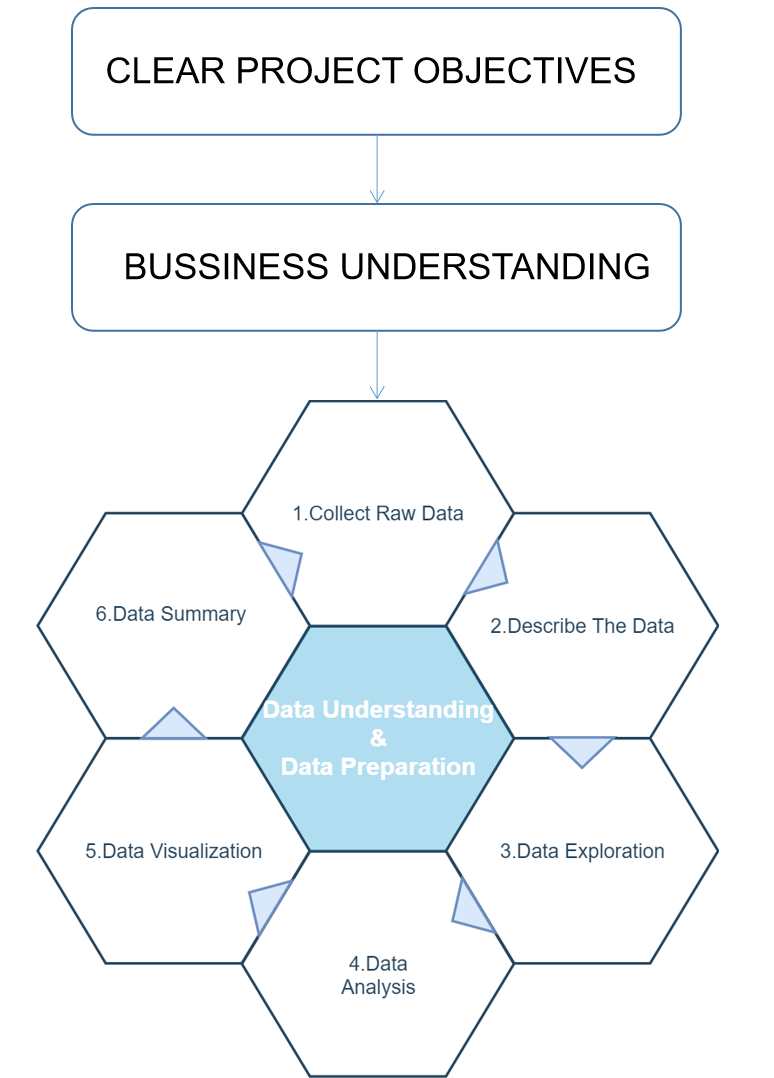
\includegraphics[width=0.6\textwidth,height=0.6\textheight]{/CSC8631_CW/Data-Management-CSC8631/new-project/data/UN1.png}

\hypertarget{project-objectives}{%
\subsection{Project objectives}\label{project-objectives}}

The purpose of this project is to explore and manage data by using R
language to sort out and filter the previously disordered raw data, and
finally present the data of an online courses ``cyber security'' from
Newcastle university to normal people and course organizers in a visual
way, this will make it easier for them to effectively understand the
concepts behind the original data.In this project, my focus is to
reflect some useful information through the correct rate of answer

\hypertarget{lets-start-with-business-understanding}{%
\subsection{Let's start with business
understanding}\label{lets-start-with-business-understanding}}

\begin{itemize}
\item
  With the development of society and science, data analysis and
  processing are more and more widely used.The focus of this project is
  to use the data from the online course of Newcastle university in the
  UK as the prototype, and to draw some effective conclusions by using
  the CRISP-DM model and EDA (exploratory data analysis).Through these
  conclusions, we hope we can improve the course arrangement in the
  future and effectively improve the quality of this course.
\item
  We hope that the course of cyber security will be well known and
  everyone can effectively acquire the knowledge they want after
  finishing this course.
\item
  In addition, the study of online courses is more free, with the
  development of the education industry, more and more people will
  choose online courses to study, which is a flexible time choice and
  high-quality education.Therefore, universities can take advantage of
  this opportunity to increase their income.
\end{itemize}

\hypertarget{data-understanding}{%
\subsection{Data Understanding}\label{data-understanding}}

\hypertarget{a-basic-overview-of-the-data}{%
\subsubsection{A basic overview of the
data}\label{a-basic-overview-of-the-data}}

\begin{itemize}
\tightlist
\item
  Our data comes from Newcastle university's online course: cyber
  security.
\item
  There are two types of data: static data and fluid data.
\item
  ``Static data'' is data that has traditionally been collected by
  certain institutions, which can be records in universities.
\item
  ``Fluid data'' is collected from everyday activities, such as swiping
  student card and logging into virtual online learning classrooms.
\item
  We have seven terms for the course data, and are ranked from
  cyber\_security 1 to cyber\_security 7, each of which means a new
  cycle for the course. These raw data recorded a lot of necessary and
  meaningful information but it needs to be filtered and processed
  before it can be used.
\end{itemize}

\hypertarget{defects-in-the-original-data}{%
\subsubsection{Defects in the original
data}\label{defects-in-the-original-data}}

\begin{itemize}
\item
  There are many null values and Unknown values in the original data. I
  think null values can be properly processed, such as elimination or
  screening, but I will keep Unknown values, because removing Unknown
  values is equivalent to reducing the sample size and affecting the
  authenticity of samples
\item
  Some of the CSV files in the original data don't give me enough
  information to process efficiently
\item
  The raw data itself cannot be directly used as the input values
  presented in the visual diagram. We need to process the data into the
  way we want it to be before screening it to get the diagram we want
\end{itemize}

\hypertarget{data-preprocessing}{%
\subsubsection{Data preprocessing}\label{data-preprocessing}}

\begin{itemize}
\item
  When I look at the given set of raw data, I finally chose 3 of them as
  the main object of processing the data, they are: ``enrolments'',
  ``question response'', and ``step activity''.(You will see the
  preprocessing results of this data in the folder I uploaded.)
\item
  My ``Enrolments'' data processing method is just to merge seven
  semesters of data and delete duplicate learner\_id's information 
\item
  In this project, what needs to be analyzed and reflected is the
  learning situation of students in this online course.In my opinion,
  the quality of students' listening in this course can be judged by
  calculating the accuracy rate of each student in answering the
  questions. 
\item
  Therefore, when preprocessing the data of ``question response'' and
  ``step activity'', I used ``hash key'' to bind the title number and
  the student number together, so as to generate all the answer data
  under the student information. In addition, I calculated several new
  variable values with the original data, such as:``Average time
  interval for each submission'',``Total number of attempts'',``The
  correct number'',``The total number of questions completed''.
\item
  Take the data preprocessing of question response as an example: 
\end{itemize}

\begin{longtable}[]{@{}llllllllll@{}}
\toprule
learner\_id & quiz\_question & Average time interval & week\_number &
first attempt & last attempt & Total attempts & correct & wrong &
correct rate\tabularnewline
\midrule
\endhead
000a49d0-39c8-4cef & 1.7.1 & 0 & 1 & 2016/9/14 15:08 & 2016/9/14 15:08 &
1 & 1 & & 0 1\tabularnewline
000a49d0-39c8-4cef & 1.7.2 & 0 & 1 & 2016/9/14 15:09 & 2016/9/14 15:09 &
1 & 1 & & 0 1\tabularnewline
000a49d0-39c8-4cef & 1.7.3 & 0 & 1 & 2016/9/14 15:10 & 2016/9/14 15:10 &
1 & 1 & & 0 1\tabularnewline
000a49d0-39c8-4cef & 1.7.4 & 0 & 1 & 2016/9/14 15:11 & 2016/9/14 15:11 &
1 & 1 & & 0 1\tabularnewline
000a49d0-39c8-4cef & 1.7.5 & 0 & 1 & 2016/9/14 15:11 & 2016/9/14 15:11 &
1 & 1 & & 0 1\tabularnewline
000a49d0-39c8-4cef & 1.7.6 & 14 & 1 & 2016/9/14 15:12 & 2016/9/14 15:12
& 3 & 1 & & 2 0.33\tabularnewline
\bottomrule
\end{longtable}

\begin{itemize}
\tightlist
\item
  Taking ``question\_response.csv'' as an example, through integration,
  we can collect all the answer data under a student id into one piece,
  which will greatly enhance the usability of the original data
\end{itemize}

\hypertarget{data-visualization}{%
\subsection{Data visualization}\label{data-visualization}}

\hypertarget{enrolments}{%
\subsubsection{Enrolments}\label{enrolments}}

\begin{itemize}
\tightlist
\item
  With data we have processed previously, we can make the following
  chart of Student enrollment information with ggplot2.
\end{itemize}

\includegraphics[width=600px,height=400]{report_files/figure-latex/unnamed-chunk-2-1}

\hypertarget{this-chart-shows-the-distribution-of-job-status-among-students-of-the-course}{%
\paragraph{This chart shows the distribution of job status among
students of the
course}\label{this-chart-shows-the-distribution-of-job-status-among-students-of-the-course}}

\includegraphics[width=600px,height=400]{report_files/figure-latex/unnamed-chunk-3-1}

\hypertarget{this-graph-shows-the-age-distribution-of-the-class}{%
\paragraph{This graph shows the age distribution of the
class}\label{this-graph-shows-the-age-distribution-of-the-class}}

\includegraphics[width=600px,height=400]{report_files/figure-latex/unnamed-chunk-4-1}

\hypertarget{this-graph-shows-the-gender-distribution-of-the-class}{%
\paragraph{This graph shows the gender distribution of the
class}\label{this-graph-shows-the-gender-distribution-of-the-class}}

\hypertarget{introduce-shiny-analysis-question-response}{%
\subsubsection{Introduce ``shiny'' analysis ``question
response''}\label{introduce-shiny-analysis-question-response}}

\begin{itemize}
\tightlist
\item
  In this project, we introduced the use of shiny, shiny is an R package
  that makes it easy to build interactive web apps straight from r. I
  will briefly introduce the structure of my shiny app through the
  processing of ``question response''. 
\item
  With the help of shiny, we can make interactive visual data, just like
  what I demonstrated in the presentation. We can choose the term number
  by selecting the filter bar, and we can integrate the question
  response data of all the terms for unified calculation.The
  visualization result will be the correct rate of the students with
  different characteristics. 
\item
  By filtering the data, we can obtain the histograms we want. Through
  these histograms, we can see the correct rate of students with
  different characteristics in different semesters.
\end{itemize}

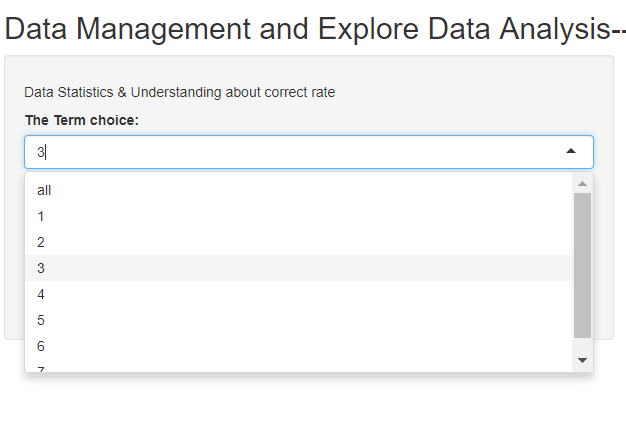
\includegraphics[width=0.4\textwidth,height=1\textheight]{/CSC8631_CW/Data-Management-CSC8631/new-project/data/UN5.png}

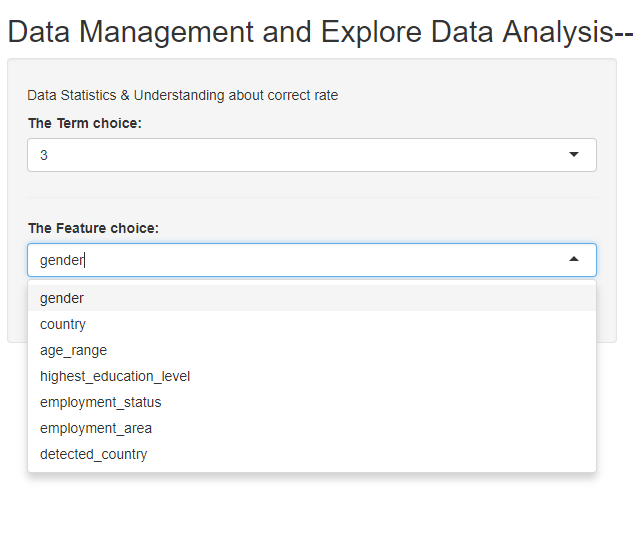
\includegraphics[width=0.4\textwidth,height=1\textheight]{/CSC8631_CW/Data-Management-CSC8631/new-project/data/UN6.png}

\begin{itemize}
\tightlist
\item
  Here, we choose data from all semesters to analyze the relationship
  between students' correct answer rate and their own characteristics
  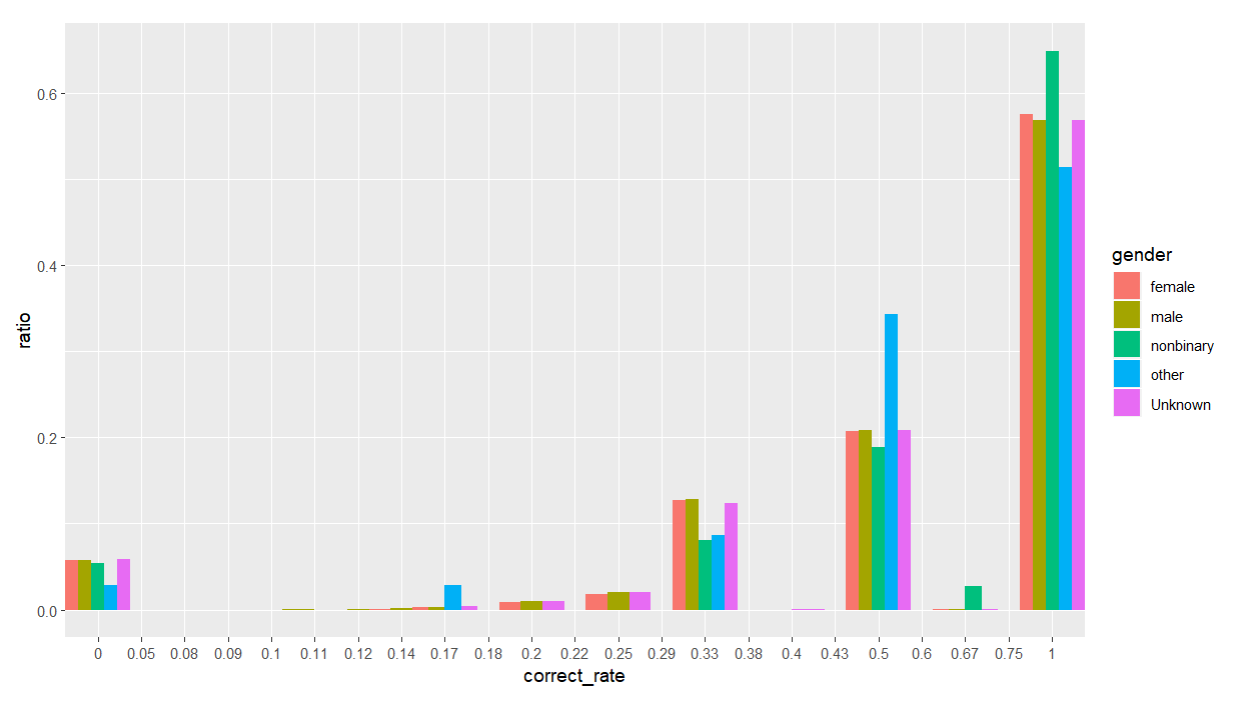
\includegraphics[width=1\textwidth,height=1\textheight]{/CSC8631_CW/Data-Management-CSC8631/new-project/data/UN7.png}
\end{itemize}

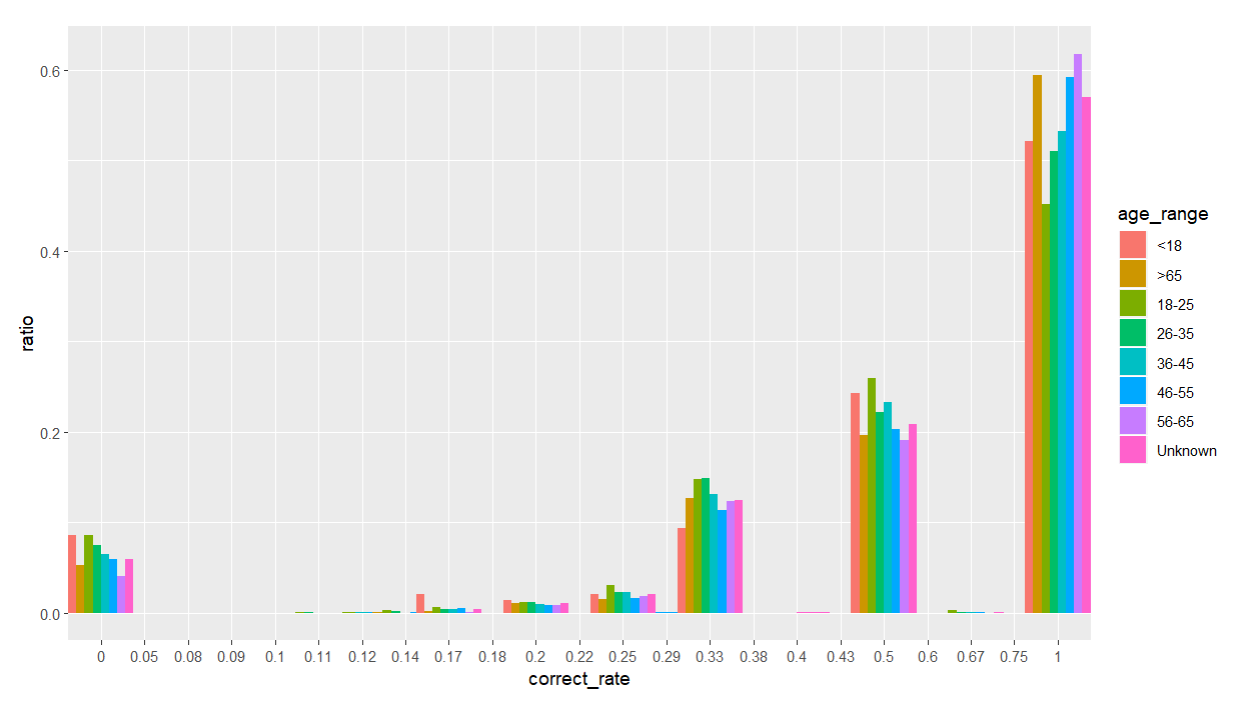
\includegraphics[width=1\textwidth,height=1\textheight]{/CSC8631_CW/Data-Management-CSC8631/new-project/data/UN8.png}

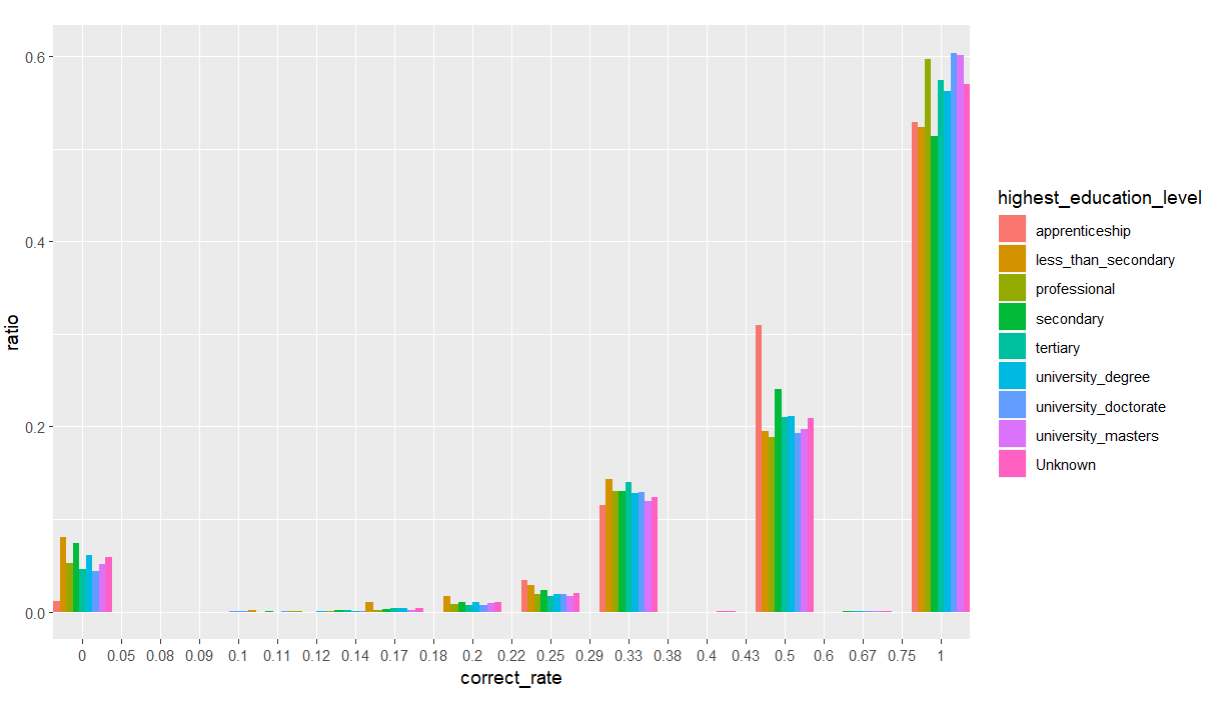
\includegraphics[width=1\textwidth,height=1\textheight]{/CSC8631_CW/Data-Management-CSC8631/new-project/data/UN9.png}

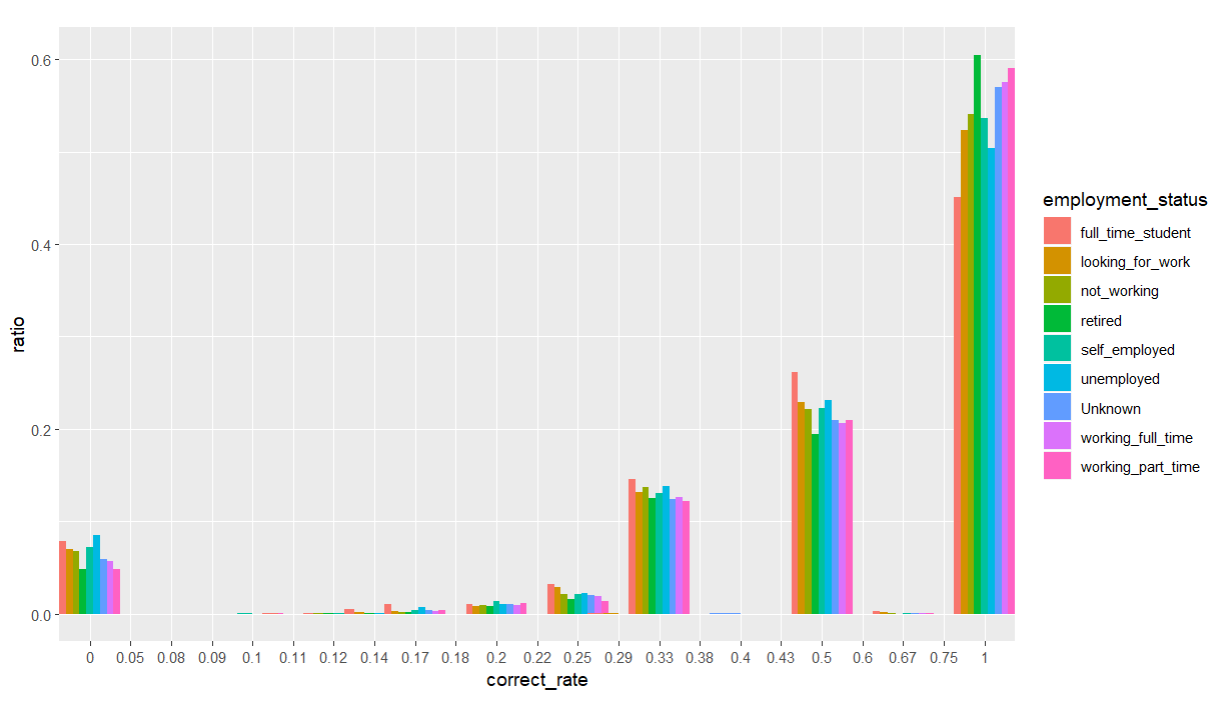
\includegraphics[width=1\textwidth,height=1\textheight]{/CSC8631_CW/Data-Management-CSC8631/new-project/data/UN10.png}

\begin{itemize}
\tightlist
\item
  I think the quality of the students' answers reflects how much they
  have learned in this online course.By the result of processing these
  data with the ``shiny'', the course organizer and the new students who
  want to attend the class can refer to the data and make decisions.
\end{itemize}

\hypertarget{data-summary}{%
\subsubsection{Data Summary}\label{data-summary}}

\begin{itemize}
\tightlist
\item
  With the help of ``shiny'', we can draw the following conclusions from
  the interactive visualized data:

  1.The accuracy rate of female students was basically the same as that
  of male students. 2.The average correct answer rate is related to
  highest education level. 3.Accuracy is related to age distribution.
  4.Correct rate was related to employment status, with those who had
  full-time and part-time jobs and those who had retired having higher
  accuracy 5.The average correct answer rate has no relationship with
  which semester cycle of the course. 6.The average correct answer rate
  is related to the working area of the occupation. 
\end{itemize}

\hypertarget{future-work}{%
\subsection{Future Work}\label{future-work}}

\begin{itemize}
\tightlist
\item
  We now have visualized data, and we need to extract key information
  from the fuzzy conclusions to help future recruits or course
  organizers make decisions
\end{itemize}

\hypertarget{deficiencies-of-this-project}{%
\subsubsection{Deficiencies of this
project}\label{deficiencies-of-this-project}}

\begin{itemize}
\tightlist
\item
  A large part of the data result after processing is still discrete
  data, which cannot be directly used for the next modeling. We need to
  consider how to solve this problem.
\item
  Because of my limited programming ability, there are many things that
  can be improved, such as ``shiny'' embedded in rmarkdown HTML,
  ``shiny'' dynamic return value and so on.It is even possible to find
  out the user group of this course and analyze the user characteristics
  by establishing the feature combination, so as to further develop the
  course plan.
\end{itemize}

\hypertarget{after-this-project-the-next-steps-will-be}{%
\subsection{After this project, the next steps will
be:}\label{after-this-project-the-next-steps-will-be}}

\hypertarget{modelling}{%
\paragraph{\texorpdfstring{Modelling }{Modelling  }}\label{modelling}}

\hypertarget{evaluation}{%
\paragraph{\texorpdfstring{Evaluation
}{Evaluation  }}\label{evaluation}}

\hypertarget{deploy}{%
\paragraph{\texorpdfstring{Deploy }{Deploy  }}\label{deploy}}

, etc.


\end{document}
